\chapter{Introducción a las ecuaciones diferenciales $\; \divideontimes$}
\chaptermark{Intro. Ecuaciones Diferenciales}

\section{?`Qué son las ecuaciones diferenciales?}

Una ecuación diferencial es una ecuación matemática que relaciona una función con sus derivadas. En las matemáticas aplicadas, las funciones usualmente representan cantidades físicas, las derivadas representan sus razones de cambio, y la ecuación define la relación entre ellas. Como estas relaciones son muy comunes, las ecuaciones diferenciales juegan un rol primordial en diversas disciplinas, incluyendo la física, la ingeniería, la química, la economía, y la biología.

En las matemáticas puras, las ecuaciones diferenciales se estudian desde perspectivas diferentes, la mayoría concernientes al conjunto de las soluciones de las funciones que satisfacen la ecuación. Solo las ecuaciones diferenciales más simples se pueden resolver mediante fórmulas explícitas; sin embargo, se pueden determinar algunas propiedades de las soluciones de una cierta ecuación diferencial sin hallar su forma exacta. Si la solución exacta no puede hallarse, esta puede obtenerse numéricamente, mediante una aproximación usando ordenadores. 

Las ecuaciones diferenciales pueden dividirse en varios tipos. Aparte de describir las propiedades de la ecuación en si, las clases de las ecuaciones diferenciales pueden ayudar a buscar la elección de la aproximación a una solución. Es muy común que estas distinciones incluyan si la ecuación es: Ordinaria/Derivadas Parciales, Lineal/No lineal, y Homogénea/Inhomogénea. Esta lista es demasiado grande; hay muchas otras propiedades y subclases de ecuaciones diferenciales las cuales pueden ser muy útiles en contextos específicos.

Una ecuación diferencial ordinaria (EDO) es una ecuación que contiene una función de una variable independiente y sus derivadas. El término ``ordinaria'' se usa en contraste con la ecuación en derivadas parciales (`concepto que no hemos estudiado porque forma parte del cálculo con funciones de varias variables') la cual puede ser respecto a más de una variable independiente.

Las ecuaciones diferenciales lineales, las cuales tienen soluciones que pueden sumarse y ser multiplicadas por coeficientes, están bien definidas y comprendidas, y tienen soluciones exactas que pueden hallarse. En contraste, las EDOs cuyas soluciones no pueden sumarse son no lineales, y su solución es más intrincada, y muy pocas veces pueden hallarse en forma exacta de funciones elementales: las soluciones suelen obtenerse en forma de series o forma integral. Los métodos numéricos y gráficos para EDOs, pueden realizarse manualmente o mediante ordenadores, se pueden aproximar las soluciones de las EDOs y su resultado puede ser muy útil, muchas veces suficientes como para prescindir de la solución exacta y analítica.


\vspace{4mm}

APLICACIONES:

\vspace{3mm}

El estudio de ecuaciones diferenciales es un campo extenso en matemáticas puras y aplicadas, en física y en la ingeniería. Todas estas disciplinas se interesan en las propiedades de ecuaciones diferenciales de varios tipos. 

Las matemáticas puras se focalizan en la existencia y unicidad de las soluciones, mientras que las matemáticas aplicadas enfatizan la justificación rigurosa de los métodos de aproximación de las soluciones. Las ecuaciones diferenciales juegan un rol muy importante en el modelado virtual de cualquier proceso físico, técnico, o biológico, por ejemplo, tanto el movimiento celeste, como el diseño de un puente, o la interacción entre neuronas. Las ecuaciones diferenciales que se plantean para resolver problemas de la vida real, no necesariamente son resolubles directamente, es decir, sus soluciones no tienen una expresión en forma cerrada. Cuando sucede esto, las soluciones se pueden aproximar usando métodos numéricos.

Muchas leyes de la física y la química se formalizan con ecuaciones diferenciales. 

En biología y economía, las ecuaciones diferenciales se utilizan para el modelado del comportamiento de sistemas complejos. 

La teoría matemática de las ecuaciones diferenciales se desarrolló inicialmente con las ciencias donde las ecuaciones se originaban y donde se encontraban resultados para las aplicaciones. Sin embargo, algunas veces se originaban problemas diversos en campos científicos distintos, de los cuales resultaban ecuaciones diferenciales idénticas. Esto sucedía porque, detrás de la teoría matemática de las ecuaciones, puede verse un principio unificado detrás de los fenómenos. Como por ejemplo, si se considera la propagación de la luz y el sonido en la atmósfera, y de las ondas sobre la superficie de un estanque. Todos estos fenómenos pueden describirse con la misma ecuación en derivadas parciales de segundo orden, `la ecuación de onda', la cual nos permite pensar a la luz y al sonido como formas de onda, y en forma similar a las ondas en el agua. 

La conducción de calor, la teoría que fue desarrollada por Joseph Fourier, está gobernada por otra ecuación en derivadas parciales de segundo orden, `la ecuación de calor'. Resulta que muchos procesos de difusión, aunque aparentan ser diferentes, están descritos por la misma ecuación. 

\footnotesize{\textcolor{gris}{En física, las ecuaciones de campo de Einstein (conocidas como EFE, por Einstein Field Equations) son un conjunto de diez ecuaciones diferenciales de segundo grado en derivadas parciales de la tepría de la relatividad general de Albert Einstein que describen la interacción fundamental de la gravitación como resultado de que el espacio-tiempo está siendo curvado por la materia y ya energía. En el límite clásico no-relativista, esto es, a velocidades pequeñas  comparadas con la luz y campos gravitacionales relativamente débiles, las ecuaciones de campo de Einstein se reducen a la ecuación de Poisson para el campo gravitatorio, que es equivalente a la ley de gravitación de Newton}}\normalsize{.}

\rightline{\textcolor{gris}{Fuente: Wikipedia}}


	\begin{figure}[H]
 		\centering
		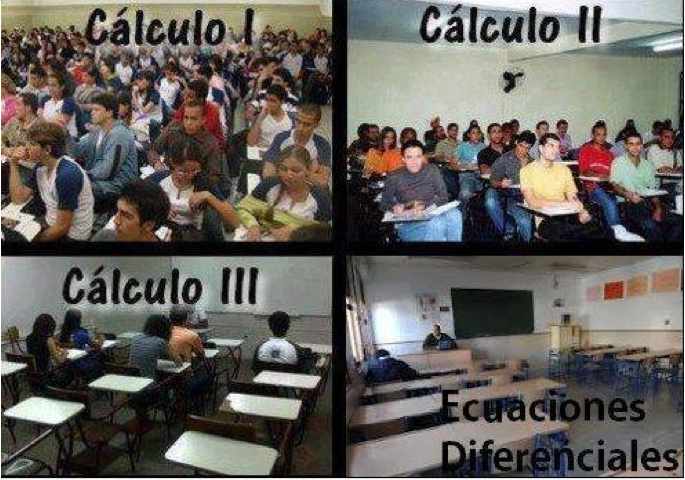
\includegraphics[width=1\textwidth]{imagenes/imagenes09/T09IM01.png}
	\end{figure}


\section{Ecuaciones diferenciales ordinarias}
	
	Sea $y=f(x)$, vamos a estudiar las ecuaciones donde intervienen la variable $x$, la función $y\;$ y alguna de sus derivadas $y';\; y''; \; y'''; \; \cdots$. Ejemplos de este tipo de ecuaciones son:
	$\quad xy'= y\; ; \qquad y''=y\; y'\; ; \qquad (y'')^2=\dfrac {x+y'}{1+x^2}$
	
\begin{defi}
Llamamos Ecuación Diferencial Ordinaria (EDO) a una ecuación el que intervengan la variable independiente $x$, una función $y(x)$ y una o varias derivadas de $y(x)$.	
\end{defi}

\begin{defi}
Llamamos `orden' de una EDO al orden de la mayor derivada que interviene en la ecuación. 
\end{defi}

Ejemplos: $\quad 2x+y\; y'=0 \text{ (orden 1) }\; ; \quad x^2 \dfrac {\dd^3 y}{\dd x^3}- \left( \dfrac {\dd y}{\dd x} \right)^4=1 \text{ (orden 3) }\; ; \quad  \dfrac {\dd^2 y}{\dd x^2}\; \cos x + \cos y =0 \text{ (orden 2) } $

Además,

\begin{defi}
Una EDO de orden `$n$' es `lineal' si se puede escribir en la forma:

\begin{equation}
	a_n(x)\; \dfrac {\dd^n y}{\dd x^n}+a_{n-1}(x)\; \dfrac {\dd^{n-1} y}{\dd x^{n-1}}+ \cdots + a_1(x)\;  \dfrac {\dd y}{\dd x}+a_0(x)\; y=b(x)
\end{equation}	
donde $a_i$ y $b$ solo dependen de $x$
\end{defi}

Ejemplos de EDO lineales:

$\sin x \; y''+y=e^x\; ; \quad \dfrac {1}{1+x^2}\; y'''+ (x^4-1)\; y=0\; ; \quad x\; \dfrac {\dd^4 y}{\dd x^4}+ x^2 \; \dfrac {\dd^2 y}{\dd x^2}+x^4\; y = x$

En cambio, no son EDO lineales:

$y\; y'=1;\qquad  \left( \dfrac{\dd y}{\dd x} \right)^2+y=0; \qquad \cos x\; \dfrac {\dd y}{\dd x}+\mathrm{ln} y=x\; \cos y$

\begin{defi}
Dada una EDO de orden $n$, llamamos `solución'	de la EDO a una función $y=f(x)$ definida en un intervalo $I$, de forma que cuando sustituimos $y=f(x)$ y sus derivadas en la EDO, ésta se verifica en todo $I$.
\end{defi}

\begin{ejem}
Consideremos la EDO $\quad y'+xy=x\; $	. Es fácil comprobar que la función $y=f(x)=1+e^{-{x^2}/2}\; $ es solución de esta EDO en todo $\mathbb R$, pero, la función $y=g(x)=1+k\cdot e^{-{x^2}/2}\; \; \text{ con } k\in \mathbb R \; $ también lo es.. Es decir, esta EDO tiene infinitas soluciones en $\mathbb R$.

Se recomienda al lector que compruebe lo dicho anteriormente.
\end{ejem}

\begin{ejem}
Para la EDO $\; y''+y=0\; $, las funciones $y=\sin x$ e $y=\cos x$ son soluciones en todo $\mathbb R$. Y, en general, dadas dos constantes $c_1, c_2 \in \mathbb R$, la función $y=c_1\; \sin x + c_2 \; \cos x$ también es solución en todo $\mathbb R$.

Se recomienda al lector que compruebe lo dicho anteriormente.
\end{ejem}

\begin{ejem}
Para la EDO $\; y'\; y^2=0 \;$	, la función $y=\dfrac 1 x$ es solución, pero en $\mathbb R^+$

Se recomienda al lector que compruebe lo dicho anteriormente.
\end{ejem}

Con los ejemplos vistos anteriormente, el conjunto de todas las soluciones de una EDO puede ser infinito. En ocasiones, nos interesa conocer solamente alguna de esas soluciones y no todas, por lo que se prefijan algunas condiciones previas a la solución buscada:

\begin{defi}{Problema de los Valores Iniciales.}

Dada una EDO de orden $n$ en un intervalo $I$ y un punto $x_0\in I$, llamamos `problema de los valores iniciales' (PVI, en lo que sigue) al problema de encontrar las soluciones de la EDO en $I$ y que además satisfagan las condiciones iniciales impuestas de antemano:

\begin{equation*}
	y(x_0)=c_0; \; y'(x_0)=c_1; \; y''(x_0)=c_2; \; \cdots ; \; y^{n-1}(x_0)=c_{n-1}
\end{equation*}

donde los $c_i$ son números prefijados.
\end{defi}

\begin{ejem}.

--- El problema PVI $\; \begin{cases} 2y\; y'=e^x \\ y(0)=0 \end{cases}\; $. Tiene como solución la función $y=e^{x/2}\; $. Puede comprobarse que es la única solución que admite el problema.

--- El problema PVI $\; \begin{cases} 2y\; y'=e^x \\ y(0)=-1 \end{cases}\; $, tiene como única solución $y=-e^{x/2}$. Compruébese.

--- La EDO de segundo orden $y''-y=x$ tiene por soluciones todas las funciones de la forma $y=-x+c_1 e^x+c_2 e^{-x} \; \forall c_1, c_2 \in \mathbb R \; $, Así, el PVI dado por $\; \begin{cases} 2y \; y'=e^x \\ y(1)=0; \; y'(1)=0 \end{cases}\; $, tiene como íunica solución $y=-x+e^{x-1}$. Compruébese.

Aunque en los ejemplos anteriores los PVI tienen solución única, pude haber problemas PVI en que hayan más de una solución.
\end{ejem}

\section{Modelos matemáticos de problemas de ciencia}

En muchas ocasiones es deseable describir en términos matemáticos el comportamiento de algunos sistemas o fenómenos de la vida real, tanto de tipo físico, químico, sociológico, económico... La descripción matemática de un sistema de fenómenos se llama `modelo matemático' y se construye con ciertos objetivos, como el de entender que ocurrirá en el futuro o que ocurrió en el pasado. Por ejemplo, podemos desear entender los mecanismos de cierto ecosistema al estudiar el crecimiento de la población animal en ese sistema, o podemos desear datar fósiles y analizar el decaimiento de una sustancia radiactiva ya sea en el fósil o en el estrato en que éste fue descubierto. 

Para la realización de un modelo matemático sobre un sistema, primero hay que identificar todas las variables que ocasionan que el sistema cambie y posteriormente establecer de qué manera estas variables afectan al sistema. Es claro que cuantas más variables que afectan al sistema se añadan mejor resolución tendrá el modelo que se obtenga. Sin embargo, el modelo será cada vez más complejo cuantas más variables entren en juego. Por ello, a veces un modelo de baja resolución (es decir, con pocas variables) es suficiente para determinar de forma aproximada la solución de nuestro problema. 

A continuación estudiaremos algunos modelos matemáticos clásicos en diferentes áreas de las Ciencias.

\subsection{Dinámica poblacional}

Dinámica poblacional. 
El economista Thomas Malthus hizo uno de los primeros intentos para modelar el crecimiento de una población. Así, supuso que la razón de la población en un cierto tiempo $t$ es proporcional a la población total en ese tiempo. Es decir, si llamamos $P(t)$ a la población en el tiempo $t$ entonces se obtiene que 

\begin{equation*}
	\dfrac {\dd P}{\dd t}=k\; P\; ,
\end{equation*}

donde $k$ es una constante que depende de la población estudiada.

Aunque este modelo es de baja resolución, aún así sigue siendo útil para el estudio de algunas poblaciones a tiempo corto, como, por ejemplo, poblaciones de cultivos de bacterias. 


\subsection{Decaimiento radiactivo}    


El núcleo de algunos átomos están formados por combinaciones de protones y neutrones inestables, es decir, los átomos se desintegran o se convierten en átomos de otras sustancias. En estos casos se dice que los núcleos son radiactivos. Por ejemplo, el radio $^{ 226 }{ Ra }$, intensamente radiactivo, se transforma en gas radón $^{ 222 }{ Rn }$.
 
Para modelar el fenómeno de decaimiento radiactivo, dada una cantidad $A(t)$ de una sustancia en el tiempo $t$, se supone que la razón con la que los núcleos se desintegran es proporcional a la cantidad existente, esto es, 
\begin{equation*}
	\dfrac {\dd A}{\dd t}= k\; A\; ,
\end{equation*}

con $k$ una constante que depende de la sustancia estudiada. 

\subsection{Ley de calentamiento-enfriamiento de Newton}
  
La ley empírica de enfriamiento/calentamiento de Newton establece que la rapidez con la que cambia la temperatura de un cuerpo es proporcional a la diferencia entre la temperatura del cuerpo y la del medio que lo rodea (la temperatura ambiente). 
 
Si denotamos por $T(t)$ a la temperatura del cuerpo en el tiempo $t$ y $T_a$ a la temperatura del ambiente, entonces, la ley de enfriamiento/calentamiento de Newton determina que 
  
  \begin{equation*}
  	\dfrac {\dd T}{\dd t}= k\; \left( T(t)-T_a \right)\; ,
  \end{equation*}
  
donde k es la constante de proporcionalidad. 

\subsection{Reacciones químicas} 
  
En algunas reacciones químicas la rapidez con la que las moléculas de una sustancia $A$ se descomponen es proporcional a la cantidad de sustancia que queda sin reaccionar. Así, si llamamos $c(t)$ a la cantidad de la sustancia $A$ en el tiempo $t$ entonces 
  
 \begin{equation*}
 	\dfrac {\dd c(t)}{\dd t}= k\;( A\;- \; c(t)) ,
 \end{equation*} 
    
donde k es una constante (dependiente de la sustancia A).
  
   
Un ejemplo de este tipo, llamada reacción de primer orden, está dada por la conversión del cloruro de terbutilo $(CH_3)_3CCl$ en alcohol t-butílico $(CH_3)_3COH$: 
   
\begin{equation*}
	(CH_3)_3CCl \; + \; NaOH \longrightarrow (CH_3)_3COH\; + \; NaCl
\end{equation*}
   
   Solo la concentración de cloruro de terbutilo controla la rapidez de la reacción. 
   
   Sin embargo, en la reacción 
   
   \begin{equation*}
   	CH_3Cl + NaOH \longrightarrow  CH_3OH + NaCl \; ,
   \end{equation*}
   
la razón con la que avanza la reacción es proporcional al producto de las concentraciones de cloruro de metilo $CH_3Cl$ y de hidróxido de sodio $NaCl$ que quedan. 
   
   Para describir en general una reacción de este tipo, conocida como reacción de segundo orden, supongamos que se combina una molécula de una sustancia $A$ con una molécula de una sustancia $B$ para formar una molécula de una sustancia $C$ (más otras sustancias). Si $c(t)$ denota la cantidad de la sustancia $C$ que se ha formado en el tiempo $t$ y si $a_0,\; b_0$ son, respectivamente, las cantidades de las sustancias $A$ y $B$ en el momento inicial $t = 0$, entonces las cantidades de $A$ y $B$ en tiempo $t$ son $a_0- c(t)$ y $b_0- c(t)$, respectivamente. Así, la razón de formación de $C$ está dada por 
   
\begin{equation*}
	\frac {\dd c}{\dd t}=k(a_0-c)(b_0-c)\; ,
\end{equation*} 
   
donde k es una constante de proporcionalidad. 

\subsection{Mezclas} 
   
   Supongamos que en un tanque mezclador tenemos $300$ litros de agua con sal. Por otro lado, un grifo de entrada introduce $3$ litros de agua por minuto, que tiene una concentración de $2$ gramos por litro. La solución bien mezclada sale del tanque con la misma rapidez de $3$ litros por minuto. 
   
De esta manera, si denotamos por $A(t)$ a la cantidad de sal en el tanque al tiempo $t$, entonces la razón con la que $A(t)$ cambia viene dada por 
   
   \begin{equation*}
   	\dfrac {\dd A}{\dd t}= \text{ (razón de entrada de sal)-(razón de salida de sal)}\; .
   \end{equation*}
   
La razón de entrada de sal es de $(2g/l) \cdot (3l/min) = 6g/min$. Por otra parte, ya que la cantidad de agua en el tanque es constantemente de $300$ litros, la 
razón de salida de sal es de $\displaystyle \left(\dfrac {A(t)}{300}\; g/l \right) \cdot \left( 3 \; l/min \right)=\dfrac {A(t)}{100}\; g/min$
   
De esta manera, 
   
   \begin{equation*}
   	\dfrac {\dd A}{\dd t}=6-\dfrac {A}{100}
   \end{equation*}
   

\subsection{Cuerpos en caída y resistencia del aire}
   
Aunque a un cuerpo en caída en el vacío solo le afecta la fuerza de la gravedad, en general, cuando no se encuentra en el vacío, el aire ejerce una resistencia al movimiento en la caída de un cuerpo. 
   
   Así , el peso del cuerpo es una fuerza que actúa en la dirección de  caída, mientras que la resistencia del aire actúa en dirección opuesta. La fuerza $F_r$ dada por la resistencia del aire se denomina amortiguamiento viscoso y es proporcional a la velocidad del cuerpo, esto es, $F_r = k\; v$, donde $k$ es una constante que depende del cuerpo y $v$ su velocidad. 
   
	La segunda ley del movimiento de Newton determina que la suma de las fuerzas ejercidas sobre el cuerpo es igual a su masa $m$ por su aceleración $a=\dfrac {\dd v}{\dd t}$, es decir, 
   
\begin{equation*}
	m\; \dfrac {\dd v}{\dd t} = m\; g - k\; v\;;
\end{equation*} 
   
donde $g$ es la aceleración de la gravedad.
   
   O equivalentemente, si denotamos por $s(t)$ al espacio recorrido en el tiempo t entonces 
   
 \begin{equation*}
 	m\; \dfrac {\dd^2 s}{\dd t^2} = m\; g - k\; \dfrac {\dd s}{\dd t}
 \end{equation*} 
 
 \vspace{3mm}
 
 \emph{La resolución de estas ecuaciones diferenciales son, en primera aproximación, una solución a los problemas planteados.}
 \section{EDOs de primer orden}
 
 En esta sección estudiaremos algunas EDO de primer orden. Hay que tener en cuenta que, en ocasiones, la solución $y(x)$ del problema aparecerá en forma implícita y en algunos casos no será posible despejarla de la ecuación:

$y^2+2xy+x^2=0;\to y\;  \text { despejable }; \quad
y+\cos y=x^3-1; \to y\;  \text { no despejable }$


\subsection{EDOs separables}

\begin{defi}
Decimos que una EDO de primer orden es `separable' o que tiene variables separables se se puede escribir en la forma: $\displaystyle \quad  \boxed{\;  g(y)\; \dfrac {\dd y}{\dd x}=h(x)\;} $
\end{defi}

Por ejemplo, la EDO $y'=e^{x-2y}\; \cos x$ es `separable', pues se puede escribir como $e^{2y}\; \dfrac {\dd y}{\dd x}=e^x\; \cos x\; $;  en cambio, la EDO $y'=y^2-\sin x\; $ no es `separable'.

\vspace{2mm}

\emph{Observación:} Una ecuación del tipo $y'=f(y)\cdot g(x)$ se puede escribir como una EDO separable de la forma $\dfrac 1 {f(y)}\; \dfrac {\dd y}{\dd x} = g(x)\;$ , pero en este caso hay que tener en cuenta que $f(y)\neq 0$, además, los números $c\; / \; f(c)=0$ cumplen que la función constante $y(x)=c$ es una solución de la EDO pues al sustituir en la ecuación original la verifican.

Así, p.e., la EDO $\; y'=(1-y^2)\; x^2\; $ es separable, se puede escribir en la forma $\frac 1 {1-y^2}\; \frac {\dd y}{\dd x}= x^2\;$. Hay que tener en cuenta, en esta ocasión, que las funciones $y(x)=1$ e $y(x)=-1$ son dos soluciones de la EDO original (soluciones de $1-y^2=0$).

\begin{teor}{Resolución EDOs separables.}

	Dada la EDO: $\displaystyle \quad  g(y)\; \dfrac {\dd y}{\dd x}=h(x)\; $ basta con escribirla en la forma: $\; g(y)\; \dd y = h(x)\; \dd x$ e integrar a ambos lados de la igualdad:
	\begin{equation*}
		\boxed{\; \int g(y)\; \dd y = \int h(x)\; \dd x\; }
	\end{equation*}
	Y así se obtienen todas las soluciones de la EDO de forma implícita.
\end{teor}

\begin{ejem}
$y^2\; y'=x-2 \to y^2\; \dd y = (x-2) \; \dd x \to y^3=x^2-2x+\mathcal C \leftrightarrow y=\sqrt[3]{x^2-2x+\mathcal C}$	
\end{ejem}

\begin{ejem}
$y'=\dfrac {y}{1+x^2} \to \dfrac {\dd y}{y} = \dfrac {\dd x}{1 + x^2} \to \mathrm{ln}|y|=\arctan x + \mathcal C\; ; \quad  \forall \mathcal C_0 \in \mathbb R; $.
Recuérdese que la solución $y=0$ también es solución de la EDO (*).

Tomando exponenciales: $y=\mathcal C_0\; e^{\arctan x}$, con $ 	\mathcal C_0=e^{\mathcal C} \;$. Esta forma general, tomando $\mathcal C_0=0$ incluye la solución $y(x)=0$ (*). 
\end{ejem}

\begin{ejem}
Sea el PVI $\begin{cases} e^{x+y} \cdot  y'= x \\ y(0)=0 \end{cases}\quad$. 

La ecuación puede escribirse como $e^y\dd y=xe^{-x}\dd x$, integrando por partes (\emph{hágase}) se obtiene: $e^y=-(1+x)e^{-x}+\mathcal C$.

Imponiendo la condición inicial $y(0)=0 \to 1=-1+\mathcal C \to \mathcal C=2$. Con lo que la solución del PVI es: $e^y=-(1+x)e^{-x}+2 \leftrightarrow y=\left(2-(1+x)e^{-x}\right)$.
	
\end{ejem}

\begin{ejem}
Sea el PVI $\begin{cases}  y'= -2x y^2 \\ y(3)=1/10 \end{cases}\quad \to \dfrac {\dd y}{y^2}=-2x \dd x $. Nótese que, al dividir por $y^2$, podría ocurrir que $y(x)=0$ que es solución de la EDO pero no del PVI, no cumple la condición inicial $y(3)=1/10$-

Integrado: $-\dfrac 1 y = -x^2+\mathcal C \to y=\dfrac {1}{x^2 - \mathcal C}$. Imponiendo la condición inicial se obtiene (\emph{hágase}) $\; y=\dfrac {1}{x^2 + 1}$
\end{ejem}

\subsection{EDOs lineales de primer orden}

Son otras EDOs, de primer orden que se pueden resolver de forma sencilla

\begin{defi}
Una EDO es de primer orden `lineal' si se puede escribir en la forma:

\begin{equation*}
	\boxed{\; a_1(x)\; y' +a_0(x)\; y = b(x)\;} 
\end{equation*}	
Con $a_1, a_0, b$ funciones que solo dependen de $x$.
\end{defi}

Poe ejemplo: $y'+x^2y=e^x \cos x\; $, ó \; $e^x y' +y =x^3$, son EDO lineales de primer orden. Sin embargo, $y'+y^2=\sen x\; $ ó $\; yy'+xy=e^x$ no lo son.

\begin{defi}
Decimos que una EDO lineal de primer orden es \textbf{homogénea} si:

 $\quad b(x)=0\qquad$, es decir, $\quad  a_1(x)\; y' +a_0(x)\; y = 0$	
\end{defi}

Ejemplos de EDO lineales de primer orden homogéneas son. $\; \sin (x)\; y' + \cos(x)\; y = 0\; $ ó $\; e^x\; y'+y=0\; $ ó $\; (x^2+1) \; y'+x\; y=0$.

\begin{teor}{Resolución EDOs lineales de primer orden.}

Para resolver la ecuación $\; a_1(x)\; y' +a_0(x)\; y = b(x)\; $, primero hay que resolver la ecuación homogénea asociada $a_1(x)\; y' +a_0(x)\; y = 0\; $. Esta última EDO es `separable' y puede resolverse como lo explicado en el apartado anterior. la solución de la EDO homogénea es de la forma $\; y(x)=\mathcal{C}_0\; y_1(x)\;$ para una cierta constante $\mathcal{C}_0$.

Si $b(x) \neq 0$, las soluciones de la ecuación  $\; a_1(x)\; y' +a_0(x)\; y = b(x)\; $ serán de la forma $y(x)=u(x)\; y_1(x)$, para una cierta función $u(x)$ a determinar. Es decir, se sustituirá la constante $\mathcal{C}_o$ dada en la EDO lineal homogénea por una función $u(x)$.

Para determinar esta  $u(x)$ se sustituirá la solución $y(x)=u(x)\; y_1(x)$ sobre la ecuación original $\; a_1(x)\; y' +a_0(x)\; y = b(x)\; $ y de ahí obtendremos una ecuación de donde podremos despejar $u'(x)$. Finalmente, por integración de esta $u'(x)$ obtendremos la  $u(x)$ y, por tanto, las soluciones de la EDO lineal de primer orden. 	
\end{teor}


\begin{ejem}
	La EDO $(1+x^2)\; y' + x\; y = 0$ el lineal, de primer orden y homogénea, por lo que la podemos resolver como `separable':
	
	$\dfrac {\dd y}{y }=-\dfrac {x}{1+x^2}$. Siempre que $y \neq 0$. De hecho, $y=0$ es solución del problema. Integrando:
	
	$\mathrm{ln} |y|=-\frac 1 2 \; \mathrm{ln} (1+x^2)+\mathcal{C} \leftrightarrow y=\dfrac {\mathcal{C}_0}{\sqrt{1+x^2}}\;$. para cualquier $\mathcal{C}_0$ real; solución que incluye a $y=0$, tomando $\mathcal{C}_0=0$
\end{ejem}



\begin{ejem}
Considera la EDO lineal de primero orden: 

$\; \arctan(y)\; y'- \dfrac {2}{1+x^2}\; y=\arctan^3 (x)\; $	

Primero resolveremos la EDO homogénea: $\; \arctan(y)\; y'- \dfrac {2}{1+x^2} \; y=0\; $

La podemos escribir, para $y\neq 0$ como separable:

$\dfrac {\dd y}{y }= \dfrac {2\; \dd x} {\arctan (x) \cdot (1+x^2)}  \; $ Se trata de una integral potencial inmediata (\emph{resuélvase}). 

El resultado es: $\; y=\mathcal {C}_0 \; \arctan^2 (x)$ 

Pare encontrar las locuciones de la EDO original, $\; \arctan(y)\; y'- \dfrac {2}{1+x^2}\; y=\arctan^3 (x)\; $, consideraremos funciones de la forma: $\; y=u(x) \cdot  \arctan^2 (x)\; $ y sustituimos en la ecuación original:

$\arctan^3 (x)= \arctan (x) \cdot \left( u(x)\cdot \arctan^2 (x) \right)' \; - \; \dfrac {2}{1+x^2} \cdot \left( u(x) \cdot  \arctan^2 (x) \right) = u'\; \arctan^3 (x)$

Tenemos que $u'(x)=1 \to u(x)=x+\mathcal C$, así, la solución de la EDO inicialmente propuesta es: 
$\; y=(x+	\mathcal C)\; \arctan^2 (x)$

\end{ejem}

\begin{ejem}

Considera el PVI: $\begin{cases} xy'-x^2y=e^{x^2/2} \\ y(1)=-1 \end{cases}$

Empezamos por resolver la EDO homogénea asociada: $\; xy'-x^2y=0\; $, que puede ser escrita (separable): $\dfrac {\dd y}{y}=x\; \dd x$. Para $y\neq 0$, integrando obtenemos (\emph{compruébese}) : $\; y=\mathcal{C}_0\; e^{x^2/2} \; $ 

Las soluciones de la EDO $\; xy'-x^2y=e^{x^2/2} \; $ serán de la forma: $y=u(x)\; e^{x^2/2}\; $. Determinaremos $u(x)$ sustituyendo la solución en la ecuación inicial:

$e^{x^2/2}=xy'-x^2y=x\; \left( u(x)\; e^{x^2/2} \right)' - x^2\, \left( u(x)\; e^{-x^2/2} \right) =x\; y'(x)\; e^{x^2/2}\; $, de donde $u'(x)= \dfrac {1} {x} \to u=\mathrm{ln}|x|+\mathcal C\; $. Así, todas las soluciones de la EDO serán: 

$\; y=\left(c+\mathrm{ln}|x| \right)\; e^{x^2/2}\;$ . Imponiendo, ahora, la condición inicial $y(1)=-1 \to c=-\dfrac {1}{\sqrt{e}}\;$ (\emph{compruébese}), con lo que la solución al PVI planteado es: 
$y=\left( \dfrac {1}{\sqrt{e}} + \mathrm{ln} x  \right) \; e^{x^2/2}$

\end{ejem}

\begin{ejem}

PVI: $\begin{cases} xy'-y=\dfrac {x^2}{1+x^2} \\ y(-1)=\pi/4 \end{cases}\; $, resolvemos primero la EDO homogénea:

$xy'-y=0 \to \dfrac{\dd y}{y}= \dfrac {\dd x }{x}\; $, para $y\neq 0\; $, (\emph{compruébese}), $y=\mathcal{C}_0\; x$ 

Las soluciones de la EDO $\; xy'-y=\dfrac {x^2}{1+x^2} \; $ serán de la forma:$\; y= u(x) \cdot  x \; $. sustituyendo:
$\dfrac {x^2}{1+x^2}= xy'-y=x\; \left( u(x) \cdots x \right)' - u(x) \cdot x =u'(x) \cdot x^2$

Por tanto, $\; u'(x)=\dfrac {1}{1+x^2}  \to u(x)=\arctan x + \mathcal C$

Las soluciones de la EDO lineal de primer orden es $\; y=\left( \mathcal C + \arctan x \right)\; x\; $ . Imponiendo la condición inicial del PVI, $y(-1)=\pi/4\; $ (\emph{hágase}), la solución del problema es: $\;y=x\; \arctan x \; $

\end{ejem}



\section{EDOs lineales de segundo orden $\;\divideontimes$}

\begin{defi}
Las EDO lineales de segundo orden son de la forma:

\begin{equation*}
  \boxed{ \; a_2\; y'' + a_1	\; y' + a_0 y= b(x) \; }
\end{equation*}
	Con $a_0\neq 0, \; b_0$ constantes reales y $h(x)$ una función de $x$
\end{defi}

\begin{teor}{Resolución EDOs lineales de segundo orden homogéneas.}

Las soluciones de una EDO de segundo orden lineal homogénea $\; a_2\; y'' + a_1	\; y' + a_0 y= b(x) \;$ son de la forma: $y(x)=\mathcal{C}_1\; y_1(x)+\mathcal{C}_2\; y_2(x)\;$. Las constantes $\mathcal{C}_1, \mathcal{C}_2$ y las funciones $y_1(x), y_2(x)$ se encuentra del siguiente modo:

Considera la ecuación de segundo grado \; $a_2\;  m^2 + a_1 \; m + a_0=0\; $ y tomamos las soluciones \; $m_1,\;  m_2\; $ de esta ecuación. Ahora distinguimos tres casos según sean estos valores:

\begin{enumerate}

\item  Si $\; m_1,\; m_2\; $	son dos números reales distintos ($\Delta=a_1^4-4a_a\cdot a_0>0$), entonces:

\begin{equation*}
	y_1(x)=e^{m_1\; x} \; ;  \qquad  \qquad y_2(x)=e^{m_2\; x}
\end{equation*}

\item Si $m_1=m_2\; $,  ($\Delta=0$), entonces:

\begin{equation*}
	y_1(x)=e^{m_1\; x} \; ;  \qquad  \qquad y_2(x)=x\; e^{m_1\; x}
\end{equation*}

\item Si las raíces son complejas conjugadas ($\Delta<0$), 
$\; m_1=\alpha + \beta \; i\; $ ; $\; m_1=\alpha - \beta \; i\; $ ($\alpha, \beta in \mathbb R$), entonces:

\begin{equation*}
	y_1=e^{\alpha\; x}\; \cos (\beta\; x) \; ;  \qquad  \qquad y_2=e^{\alpha\; x}\; \sin (\beta\; x)
\end{equation*}
\end{enumerate}
\end{teor}

\vspace{4mm}

\begin{ejem}
$y''-3y'+2y=0 \to m^2-3m+2=0 \to m_1=1 \; \wedge m_2=2\; $

Entonces, las soluciones de la EDO son: $\; y=\mathcal{C}_1\; e^x +\mathcal{C}_2\; e^{2x}\; , \quad \forall \mathcal{C}_1,\mathcal{C}_2 \in \mathbb R$  	
\end{ejem}

\begin{ejem}
La EDO $\; 4y''-4y'+y=0\; $ tiene por ecuación de segundo grado asociada $\; 4m^2-4m+1=0 \to m_1=m-_2=\frac 1 2 \; $.

Las soluciones de la EDO son: $\; y=\mathcal{C}_1\; e^{x/2} + \mathcal{C}_2\;x\; e^{x/2} \; , \quad \forall \mathcal{C}_1,\mathcal{C}_2 \in \mathbb R$
\end{ejem}



\begin{ejem}
$y''-4y'+13y=0 \to m^2-4m+13=0 \to 	m=2\pm 3\; i$

Las soluciones de la EDO son $\; y= \mathcal{C}_1\; e^{2x} \cos (3x) + \mathcal{C}_2\; e^{2x} \sin  (3x) \; , \quad \forall \mathcal{C}_1,\mathcal{C}_2 \in \mathbb R$
\end{ejem}



\begin{ejem}
PVI: $\; \begin{cases} y''-4y'+5y=0 \\ y(0)=3; \; y'(0)=1 \end{cases}$

Primero resolvemos la EDO, cuyo polinomio asociado es: $,^2-4m+5=0 \to m=2\pm  i$. Por ello, las soluciones de la EDO son:
$\; y= \mathcal{C}_1\; e^{2x} \cos (x) + \mathcal{C}_2\; e^{2x} \sin  (x) \; , \quad \forall \mathcal{C}_1,\mathcal{C}_2 \in \mathbb R$

Imponiendo las condiciones iniciales: $\quad y(0)=3; \; y'(0)=1 \; $ (\emph{hágase}), obtenemos la solución de PVI: $\quad y=e^{2x}\; (3\cos x-5\sin x)$
	
\end{ejem}

\vspace{3mm}

Para la EDO lineal de segundo orden lineal tiene la forma: $\; a_2\; y'' + a_1	\; y' + a_0 y= b(x)\; $, con $\; b(x) \neq  0\; $, la solución se obtiene de otro modo, como se explica en el siguiente teorema:


\begin{teor}{Resolución EDOs lineales de segundo orden generales.}

Dada $\; a_2\; y'' + a_1	\; y' + a_0 y= b(x)\; $, primero se resuelve la ecuación homogénea asociada, es de decir: $\; a_2\; y'' + a_1	\; y' + a_0 y= 0 \; $ y se encuentran sus soluciones, del tipo: $\; y=\mathcal{C}_1\; y_1(x) +\mathcal{C}_2\; y_2(x)\; , \quad \forall \mathcal{C}_1,\mathcal{C}_2 \in \mathbb R\; $ e $y_1(x),\; y_2(x)\; $ funciones de $x$.  que se obtienen como se ha explicado en el teorema anterior.

Las soluciones de la EDO general serán de la forma $\; y= u_1(x)\; y_1(x) \; + \; u_2(x)\; y_2(x)\; $, donde las funciones $u_i$ se encuentran al resolver el sistema:

\begin{equation*}
	\begin{cases}
	u'_1(x)\; u_1(x) + u'(2)\; y_2(x)=0 \\
	u'_1(x)\; y'_1(x) + u'_2(x)\; y'_2(x)= \dfrac {b(x)}{a_2}	
	\end{cases}	
\end{equation*}

Las derivadas $u'_i(x)$ se han de integrar y ya se obtiene la solución.	
\end{teor}

\vspace{4mm}


\begin{ejem}
$y''+y'-2y=3e^x \to $ Primero resolvemos la EDO homogénea: 

$y''+y'-2y=0 \to m^2+m-2=0 \to m_1=1 \; \wedge \; m_2=-2 $

Las soluciones de la EDO homogénea son:  $y=\mathcal{C}_1 e^x + \mathcal{C}_2 e^{-2x}$. Montemos el sistema:

$\begin{cases}
u'_1(x)\; e^x + u'_2(x)\; e^{-2x}=0 \\
u'_1(x)\; e^x - 2x \; u'_2(x)\; e^{-2x}= 3e^x	
\end{cases} \to $ Resolviendo el sistema (\emph{hágase}):

$u'_1(x)=1 \to u_1(x)=x + \mathcal{C}_1 ; \quad u'_2(x)=-e^{3x} \to u_2(x)=-\frac 1 3 e^{3x}+\mathcal{C}_2$. La soluciones de la EDO gral. son (\emph{hágase}):

\hspace{20mm} $y=\left( x+\mathcal{C}_1 \right)\; e^x + \left( -\frac 1 3 e^{3x} + \mathcal{C}_2 \right) \; e^{-2x}=(*)= (x+\mathcal{D}_1) \; e^x + \mathcal{C}_2\; e^{-2x}$, 

con $\mathcal{D}_1, \; \mathcal{C}_2$ constantes reales por determinar.

\rightline{\textcolor{gris}{(*) $e^{3x} \cdot e^{-2x}=e^x$}}
	
\end{ejem}



\begin{ejem}
$9y''+6y'+y=\sin x \to : \; $ EDO homogénea: $9y''+6y'+y=0 \to :\; $  Polinomio asociado: $9m^2+6m+1=0 \to m_1=m_2=-\frac 1 3 \to : \; $ Soluciones de la EDO homogénea: $y=\mathcal{C}_1 \; e^{-x/3} + \mathcal{C}_2 \; x \; e^{-x/3} \to :\; $	Sistema de ecuaciones para determinar las $u_i$:

$\begin{cases}
u'_1(x)\; e^{-x/3} + u'_2(x) \; x \; e^{-x/3} = 0 \\
-\frac 1 3 \; u'_1(x)\; e^{-x/3} - \frac 1 3 \; (x-3)\;  u'_2(x)\ e^{-x/3} = \frac {\sin x}{9} 	
\end{cases}$

Resolviendo el sistema anterior (\emph{hágase}), se obtiene:
$\quad u_1(x)=-\frac 1 9 \; x \; e^{-x/3}\; \sin x ; \quad  u'_2(x)= \frac 1 9 \; e^{x/3} \; \sin x\; $, ahora, integrando (\emph{hágase}), se obtienen las funciones $u_i$:

$u_1(x)=\mathcal{C}_1+\frac 1 {150}\;  e^{-x/3} \; \left( 3(5x-3)\cos x -(5x+12)\sin x \right)\;$

$u_2(x)=\mathcal{C}_2 - \frac 1 {30} \; e^{-x/3}\; (3\cos x-\sin x)$

Con lo que las soluciones de la EDO gral son:

\hspace{30mm} $y=\mathcal{C}_1 \; e^{-x/3}+\mathcal{C}_2 \; x \; e^{-x/3}- \frac 1 {50} \; (3\cos x + 4 \sin x)$

\end{ejem}


\begin{ejem}
	$y''+2y'+2y=e^{-x} \to y''+2y'+2y=0 \to m^2+2m+2=0 \to m=-2 \pm i$

Soluciones EDO homogénea: $y=\mathcal{C}_1 e^{-x} \cos x + \mathcal{C}_2 e^{-x} \sin x \; \to \; $ Sistema:

$\begin{cases}
u'_1(x)e^{-x} \cos x + u'_2(x) e^{-x} \sin x = 0 \\
-u'_1(x) e^{-x} (\cos x + \sin x ) + u'_2(x) e^{-x} (\cos x - \sin x )=e^{-x}	
\end{cases}$

Soluciones e integrales: $u'_1(x)=-\sin x \to u_1(x)=\mathcal{C}_1 + \cos x ; \quad u'_2(x)=\cos x \to u_2(x)=\mathcal{C}_2 +\sin x$ Y la solución de la EDO lineal de segundo orden lineal es:

\hspace{30mm} $y=e^{-x}\cdot \left( 1+ \mathcal{C}_1 \; \cos x + \mathcal{C}_2 \; \sin x \right)$ 


\end{ejem}

\begin{ejem}
	PVI: $\; \begin{cases} y''-6y'+9y=2e^3x \\ y(0)=1; \; y'(0)=-2 \end{cases}$

Resolvemos primero la EDO homogénea: $y''-6y'+9y=0 \to m^2-6m+9=0 \to m_1=m_2=3$

Soluciones de la EDO homogénea: $y=\mathcal{C}_1 \; e^{3x} + \mathcal{C}_2\; x \; e^{3x}$

Sistema: $\; \begin{cases}
 u'_1(x)\; e^{3x} + u'_2(x) x e^{3x} =0 \\
 3u'_1(x) e^{3x}+(3x+1) u'_2(x) e^{3x}=2 e^{3x}	
 \end{cases} 	\to \begin{cases}
 u'_1(x)= -2x \to u_1(x)=-x^2 + \mathcal{C}_1 \\
 u'_2(x)=2 \to u_2(x)=2x+\mathcal{C}_2	
 \end{cases}$
 
 Con todo ello, la solución de la EDO gral. es:  $\; y=e^{3x}\; (x^2+\mathcal{C}_2\; x + \mathcal{C}_1)$
 
 Finalmente, imponiendo las condiciones iniciales $y(0)=1; \; y'(0)=-2$, se obtiene, como solución de PVI:
 
 \hspace{30mm} $y=e^{3x}\; (x^2-5x+1)$
 
 \rightline{\textcolor{gris}{\emph{háganse todos los pasos que faltan.}}}

\end{ejem}



\textit{La redacción de este capítulo es copia `casi' textual de los apuntes de catedrático de apuntes del catedrático J.A. Gálvez, del departamento de geometría y topología de la universidad de Granada. Muchas gracias por compartir tu saber.}




\section{Aplicaciones de las ecuaciones diferenciales}

\rightline{\textit{Fuente: wikipedia}}

\vspace{3mm}

\textcolor{gris}{
El estudio de ecuaciones diferenciales es un campo extenso en matemáticas puras y  aplicadas, en física y en la ingeniería. Las ecuaciones diferenciales juegan un rol muy importante en el modelado virtual de cualquier proceso físico, técnico, o biológico, por ejemplo, tanto el movimiento celeste, como el diseño de un puente, o la interacción entre neuronas. Las ecuaciones diferenciales que se plantean para resolver problemas de la vida real, no necesariamente son resolubles directamente, es decir, sus soluciones no tienen una expresión en forma cerrada. Cuando sucede esto, las soluciones se pueden aproximar usando métodos numéricos.}

\textcolor{gris}{Muchas leyes de la física y la química se formalizan con ecuaciones diferenciales. En biología y economía, las ecuaciones diferenciales se utilizan para el modelado del comportamiento de sistemas complejos. La teoría matemática de las ecuaciones diferenciales se desarrolló inicialmente con las ciencias donde las ecuaciones se originaban y donde se encontraban resultados para las aplicaciones. Sin embargo, algunas veces se originaban problemas diversos en campos científicos distintos, de los cuales resultaban ecuaciones diferenciales idénticas. Esto sucedía porque, detrás de la teoría matemática de las ecuaciones, puede verse un principio unificado detrás de los fenómenos. Como por ejemplo, si se considera la propagación de la luz y el sonido en la atmósfera, y de las ondas sobre la superficie de un estanque. Todos estos fenómenos pueden describirse con la misma ecuación en derivadas parciales de segundo orden, la ecuación de onda, la cual nos permite pensar a la luz y al sonido como formas de onda, y en forma similar a las ondas en el agua. La conducción de calor, la teoría que fue desarrollada por Joseph Fourier, está gobernada por otra ecuación en derivadas parciales de segundo orden, la ecuación de calor. Resulta que muchos procesos de difusión, aunque aparentan ser diferentes, están descritos por la misma ecuación. La ecuación de Black-Scholes en las finanzas, está por ejemplo, relacionada con la ecuación del calor.}

\textcolor{gris}{\textbf{Física}}

\textcolor{gris}{•	Ecuaciones de Euler-Lagrange en mecánica clásica.}

\textcolor{gris}{•	Ecuaciones de Hamilton en mecánica clásica.}

\textcolor{gris}{•	Radiactividad en física nuclear.}

\textcolor{gris}{•	Ley de enfriamiento de Newton en termodinámica.}

\textcolor{gris}{•	Ecuación de onda.}

\textcolor{gris}{•	Ecuación de calor en termodinámica.}

\textcolor{gris}{•	Ecuación de Laplace, que define las funciones armónicas.}

\textcolor{gris}{•	Ecuación de Poisson.}

\textcolor{gris}{•	Ecuación geodésica.}

\textcolor{gris}{•	Ecuaciones de Navier-Stokes en fluidodinámica.}

\textcolor{gris}{•	Ecuación de difusión en procesos estocásticos.}

\textcolor{gris}{•	Ecuación de convección-difusión en fluidodinámica.}

\textcolor{gris}{•	Ecuaciones de Cauchy-Riemann en análisis complejo.}

\textcolor{gris}{•	Ecuación de Poisson-Boltzmann en dinámica molecular.}

\textcolor{gris}{•	Ecuaciones de Saint-Venant.}

\textcolor{gris}{•	Ecuación diferencial universal.}

\textcolor{gris}{•	Ecuaciones de Lorenz cuyas soluciones exhiben un flujo caótico.}

\textcolor{gris}{\textbf{Mecánica clásica.}}


\textcolor{gris}{Siempre que se conozca la fuerza actuante sobre una partícula, la Segunda ley de Newton es suficiente para describir el movimiento de una partícula. Una vez que están disponibles las relaciones independientes para cada fuerza que actúa sobre una partícula, se pueden sustituir en la segunda ley de Newton para obtener una ecuación diferencial ordinaria, la cual se denomina ecuación de movimiento}.

\textcolor{gris}{\textbf{Electrodinámica.}}

\textcolor{gris}{Las ecuaciones de Maxwell son un conjunto de ecuaciones en derivadas parciales que, junto con la ley de la fuerza de Lorentz , forman los fundamentos de la electrodinámica clásica, óptica clásica, y la teoría de los circuitos eléctricos. Estos campos se volvieron fundamentales en las tecnologías eléctricas, electrónicas y de comunicaciones. Las ecuaciones de Maxwell describen cómo los campos eléctrico y magnético se generan alterando uno y otro por cargas y corrientes eléctricas. Estas ecuaciones deben su nombre al físicomatemático escocés James Clerk Maxwell, quien publicó sus trabajos sobre estas ecuaciones entre 1861 y 1862.}

\textcolor{gris}{\textbf{Relatividad general.}}

\textcolor{gris}{Representación de la curvatura dada por la ecuación de campo de Einstein sobre el plano de la eclíptica de una estrella esférica: Dicha ecuación relaciona la presencia de materia con la curvatura adquirida por el espacio-tiempo.}

\textcolor{gris}{Las ecuaciones de campo de Einstein (conocidas también como "ecuaciones de Einstein") son un conjunto de diez ecuaciones en derivadas parciales de la teoría de la relatividad general donde se describe la interacción fundamental de la gravitación como un resultado de que el espacio-tiempo es curvado por la materia y la energía.}
 
\textcolor{gris}{Publicado por primera vez por Einstein en 1915 como una ecuación tensorial, las ecuaciones equiparan una curvatura espacio-tiempo local (expresada por el tensor de Einstein) con la energía y momentum local dentro del espacio-tiempo (expresado por el tensor de energía-impulso).}

\textcolor{gris}{\textbf{Mecánica cuántica.}}

\textcolor{gris}{En la mecánica cuántica, el análogo a la ley de Newton es la Ecuación de Schrödinger (una ecuación en derivadas parciales) para un sistema cuantificado (usualmente átomos, moléculas, y partículas subatómicas que pueden estar libres, ligadas, o localizadas). No es una ecuación algebraica simple, pero es, en general, una ecuación en derivadas parciales y lineal, que describe la evolución en el tiempo de una función de onda (también llamada una "función de estado").}

\textcolor{gris}{\textbf{Biología.}}
 
\textcolor{gris}{•	Ecuación de Verhulst – para el crecimiento de población biológica.}
 
\textcolor{gris}{•	Modelo de von Bertalanffy – para el crecimiento individual biológico.}
 
\textcolor{gris}{•	Dinámica de replicación – en teoría biológica.}
 
\textcolor{gris}{•	Modelo de Hodgkin y Huxley – potenciales de acción neuronal.}
	
\textcolor{gris}{\textbf{Ecuaciones predador-presa.}}

\textcolor{gris}{Las ecuaciones Lotka–Volterra, también conocidas como las ecuaciones predador-presa, son un par de ecuaciones diferenciales no lineales de primer orden frecuentemente utilizadas para describir la dinámica de sistemas biológicos en los cuales interactúan dos especies, una el predador, y la otra, la presa. }

\textcolor{gris}{\textbf{etc...}}




	